\twocolumn[
\begin{center}
\title{\color[cmyk]{1, 0.57, 0, 0.38}{\Huge\bfseries Editoriale\\}} % definisco il titolo dell'articolo
\author{\scriptsize Gabriele Trombini (mailga@fedoraonline.it)} % definisco l'autore e altre informazioni
\date{}
\end{center}
{\color[cmyk]{1, 0.46, 0, 0}\LARGE Folio - il primo numero e le nostre aspettative}\\
\maketitle
\normalsize
\doublespacing
\hfill
]
\onehalfspacing
\lettrine[lines=1, loversize=0.1, lraise=0.1]{\color[cmyk]{0.5, 0, 1, 0}\bfseries C}{}arissimi lettori,\\ 
era da parecchio tempo che avevamo in cantiere l'idea di redigere una rivista in formato PDF che parlasse di tematiche al di fuori di quelle trattate all'interno del forum tecnico.\\

Il progetto, sempre rimandato soprattutto per mancanza di tempo, ha ripreso il vigore necessario quando si è stabilito che era il momento di gettare il cuore oltre l'ostacolo.\\

Di certo non potevamo lasciarci sfuggire l'occasione fornita dal restyling del sito, per cui eccoci a presentare il primo numero (numero pilota) di questa nuova iniziativa di FedoraOnLine e del suo staff.\\

E' sicuramente un layout non definitivo, da affinare e collaudare nel tempo; una prova, quindi, per verificare la centralità del progetto rispetto alle aspettative dell'utente.\\

Non vogliamo che diventi una sovrapposizione di FedoraOnLine, pertanto ciò che tratteremo in questa sede saranno argomenti, talvolta tecnici, che descriveranno il funzionamento di programmi, del sistema e di tutte quelle particolarità che nel forum non vengono approfondite per ovvie ragioni di tempo e spazio, ma che riteniamo essere di importanza rilevante per gli utenti.\\

\begin{figure}[htbp]
\centering
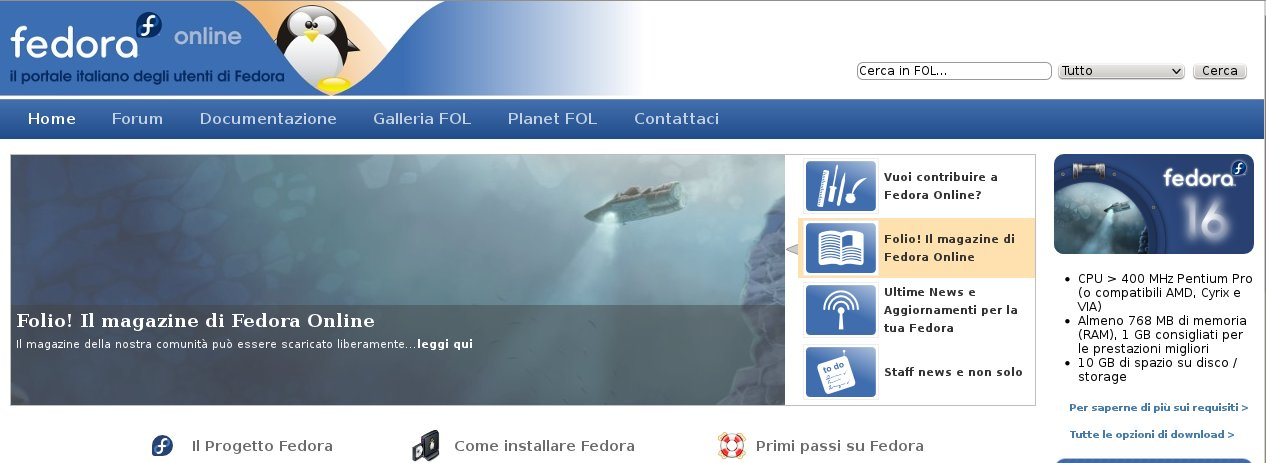
\includegraphics[scale=.20]{articoli/editoriale/immagini/fol.jpeg}
\caption{il nuovo portale FedoraOnLine\label{fig 1:Il nuovo portale FedoraOnLine}}
\end{figure}

Verranno anche portate avanti e sviluppate tematiche connesse a Fedora, al Fedora Project ed a quant'altro ruoti intorno ai sistemi GNU/Linux con l'intenzione di accorciare la distanza che intercorre tra gli utenti ed il Fedora Project, scrivendo diffusamente sulle qualità e, perchè no?, dei difetti della struttura organizzativa, conoscendo anche da vicino chi è impegnato nelle varie attività ad esso correlate.\\

Ma non solo! FedoraOnLine, tramite questa rivista, vuole cercare di ridurre quelle difficoltà che i nuovi utenti riscontrano nell'avvicinamento a GNU/linux, createsi sia per oggettive complessità tecniche sia per stereotipi che non hanno senso di esistere; in sostanza proveremo a descrivere una visione a 360 gradi dell'open source e del free software.\\

Non abbiamo mire editoriali, non siamo professionisti della carta stampata, nè vogliamo esserlo, ma questa iniziativa è rivolta a coloro, soprattutto, che hanno voglia di guardare e capire cosa ci lega ad uno sviluppatore dell'Illinois, ad un grafico dell'India e a chissà quante altre persone.\\

Basta un gesto del mouse o premere un carattere sulla tastiera affinchè i {\itshape linuxiani} si pongano delle domande.\\

Già qualche anno fa eravamo riusciti a trasformare una idea in qualcosa di buono e di utile, scrivendo un libro sulla release 9 di Fedora, che fornisse un supporto per l'avvicinamento al nostro sistema operativo.\\

\begin{figure}[htbp]
\centering
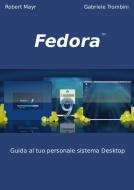
\includegraphics[scale=.55]{articoli/editoriale/immagini/libro_copertina.jpg}
\caption{Fedora 9, il libro\label{fig 2:Fedora 9, il libro}}
\end{figure}

Ovviamente siamo del tutto aperti a consigli, critiche e a correzioni da parte di chi legge ed il riferimento a cui inviare tutto ciò che vi dovesse venire in mente è {\itshape redazione@fedoraonline.it}.\\

In questo primo numero cominceremo ad introdurre il Fedora Project, descrivendone gli obiettivi e parlandone un po' con chi ne è addentro, parleremo dei motivi e dei retroscena che ci hanno portato al restyling del nostro sito, vedremo come avvicinarci alla shell Linux, approfondiremo software, illustreremo i servizi di Fedora, daremo una prima occhiata al kernel e comincieremo a studiare il sistema di packaging di Fedora, cioè gli rpm.\\

Ovviamente non potremo fare a meno di gettare uno sguardo sul futuro prossimo di Fedora, alle features annunciate per la release numero 17 la cui uscita è prevista a Maggio 2012, come da roadmap che si può trovare alla pagina {\itshape http://fedoraproject.org/wiki/Schedule}.\\

Niente altro da aggiungere, al momento, specificando, però, che l'impostazione grafica della rivista sarà soggetta a miglioramenti e che per il momento la cadenza per la pubblicazione dei numeri successivi a questo è ancora lontana dall'essere definita.\\

Il successo di questa iniziativa dipende dai nostri lettori, vi aspettiamo. 



